\chapter{Implementazione}

\section{Servizi Onion}
Nelle comuni reti internet i servizi vengono utilizzati facendo richieste basate sugli indirizzi IP pubblici, la sorgente e destinazione di un pacchetto è quindi conosciuta da tutti i dispositivi che la ricevono. 
Onion invece garantisce l'anonimato non solo agli utenti ma anche ai servizi, nascondendone l'indirizzo IP. 
Questo viene fatto tramite uno pseudonimo di lungo termine, identico in tutti i circuiti e stabile anche al un fallimento di un router \\
I principali obiettivi sono
\begin{itemize}
    \item Gli attaccanti non devono riuscire a manipolare la rete sostituendosi un servizio esistente. Questo livello di affidabilità deriva dalla criptografia asimmetrica che ci garantisce che il servizio a cui cerchiamo di connetterci sia autentico, solo lui possiede la copia privata della chiave pubblica con cui tentiamo la connessione
    \item Sicurezza dagli attacchi DoS, viene fatto tramite l'uso di più punti d'ingresso alla rete 
\end{itemize}
La creazione di un servizio onion passa per diversi punti prima di poter essere raggiungibile
\begin{enumerate}
    \item Genera una coppia di chiave pubblica e privata per identificarsi
    \item Definisce alcuni onion router come punti di ingresso nella rete, da cui riceverà le richieste dei clienti e invia loro la chiave pubblica
    \item Crea un circuito con ogni punto di ingresso
    \item Invia al servizio di lookup onion le informazioni sui punti d'ingresso e l'hash della chiave pubblica che sarà usata come hostname\ref{sec:DirectoryServers}
\end{enumerate}
Quando un utente tenta la connessione
\begin{enumerate}
    \item Inizialmente esegue il lookup del dominio tramite un directory server
    \item Successivamente sceglie un OR come tramite per il servizio e genera un circuito verso di esso, sfruttando uno specifico cookie per identificare il servizio
    \item Viene generato uno stream verso uno dei punti d'ingresso del servizio con tutte le informazioni riguardo se stesso, il nodo tramite e il cookie. Tutto viene criptato con la chiave pubblica del servizio
    \item Inizia l'handshake di Diffle-Hellman tra OP e servizio
    \item Il servizio onion a sua volta genera un circuito verso il nodo tramite per poter rispondere all'OP con la seconda parte dell'handshake
    \item Il nodo tramite collega i due circuiti generando un circuito dati bidirezionale 
\end{enumerate}
Sia il programma dell'utente che il web server non vengono modificati e non sono nemmeno a corrente che il traffico viaggia per una rete onion \cite{ChaumMixes}
\section{Onion V3}
La terza generazione di onion nasce per risolvere alcuni problemi di sicurezza. In particolare rispetto alla seconda generazione
\begin{itemize}
    \item Sono stati aggiornati i sistemi di crittografia, da SHA1/DH/RSA1024 a SHA3/ed25519/curve25519
    \item Sono stati migliorati i directory server e il directory protocol
    \item È stato cambiato il sistema di hostname. Precedentemente venivano usati i primi 80 bit dell'hash (SHA1) della chiave pubblica per creare l'hostname\footnote{un esempio \textbf{yyhws9optuwiwsns.onion}}, nella terza generazione vengono codificati in base32
    \begin{itemize}
        \item La chiave pubblica, un totale di 32 byte in ed25519
        \item Il checksum di 2 byte
        \item Un byte di versione, di default '\textbackslash x03' 
    \end{itemize}
    In totale il nuovo hostname possiede 56 caratteri\footnote{esempio l'indirizzo \emph{pg6mmjiyjmcrsslvykfwnntlaru7p5svn6y2ymmju6nubxndf4pscryd.onion}, se proviamo a decodificarlo otteniamo la stringa 79bcc625184b05194975c28b66b66b0469f7f6556fb1ac3189a79b40dda32f1f214703, come notiamo termina con 03, il byte di versione}
\end{itemize}
Inoltre l'indirizzo v3 contenendo l'intera chiave pubblica, una volta decodificato\footnotemark[2] in base32\footnote{Definito nell'RFC 3548 e 4648} ci ritorna tutte le informazioni necessarie per connettersi al servizio. \\
\cite{Torv3}

\newpage
\section{Studio delle tecnologie}
% TODO fig grammatico e migliorare la scrittura
Per creare un servizio sulla rete onion si possono usare una moltitudine di tecnologie differenti, ogni singolo aspetto necessita di effettuare delle scelte. \\
\begin{itemize}
    \item Deploy del Server, la prima scelta ricade sulla creazione del server e in particolare scegliere dove eseguire il deploy, ci sono molteplici motivi per usare un servizio cloud, tra cui la sicurezza e la facilità d'uso. Ci sono 3 principali competitor e molti altri secondari che per la maggior parte sfruttano i server di queste 3 aziende
    \begin{itemize}
        \item Microsoft Azure
        \item Google Cloud
        \item Amazon Web Service, il più importante servizio cloud, è gestito e reso disponibile da Amazon e possiede molti servizi tra cui scegliere. Per questa implementazione useremo il servizio EC2 messo a disposizione da AWS in una macchina t3.micro
    \end{itemize}
    \item SO, la seconda scelta ricade sul sistema operativo della nostra macchina. Debian in particolare ha molti vantaggi, tra cui 
    \begin{itemize}
        \item Leggerezza, affidabilità e sicurezza derivate da un sistema GNU/Linux
        \item Maggiore utilizzo in ambienti server
        \item Nessun costo aggiuntivo derivato dall'aquisto di una licenza d'uso come Windows server
    \end{itemize}
    Useremo in particolare la versione 11
    \item Web Server, abbiamo due web server principali 
    \begin{itemize}
        \item Apache httpd, il più vecchio dei due, rilasciato con licenza Apache 2.0
        \item Nginx, un web server più moderno che fornisce diversi altri strumenti oltre al web server, tra cui il proxy e load balancer, è gratuito e come httpd è open source, ha superato apache da un paio di anni. Viene anche utilizzato in container docker, ma noi lo useremo in una classica macchina virtuale.
    \end{itemize}
\end{itemize}

\newpage
\section{Creazione del servizio}

Una volta creato l'account AWS possiamo creare una macchina virtuale andando nella sezione EC2 -> Instances -> Launch Instances, durante la configurazione possiamo selezionare le opzioni che abbiamo precedentemente analizzato
\begin{enumerate}
    \item Il nome
    \item Il sistema operativo da usare, selezioniamo Debian 11 e in particolare l'architettura x86,
    \item L'istanza scelta è una semplice t3.micro con 2 vCPU e 1 GiB di memoria
    \item Una coppia di due chiavi pubblica e privata, selezioniamo o creiamo una 
    \item Successivamente è fondamentale aggiungere alla macchina i giusti security group, di default AWS non consente nessun tipo di traffico in entrata o in uscita dalla macchina
    \begin{itemize}
        \item Consentire la connessione ssh alla porta 22
        \begin{figure}[h]
            \centering
            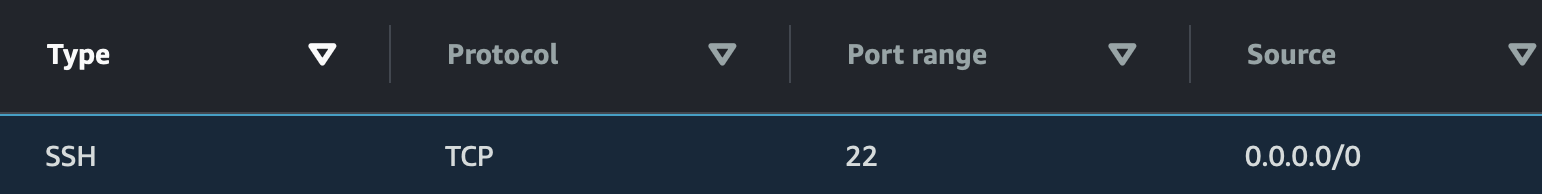
\includegraphics[width=\textwidth]{securityGroup1}
            \caption{security Group 1, ssh in entrata}
            \label{fig:sec1}
        \end{figure}
        
        \item Consentire il traffico TCP in uscita
        \begin{figure}[h]
            \centering
            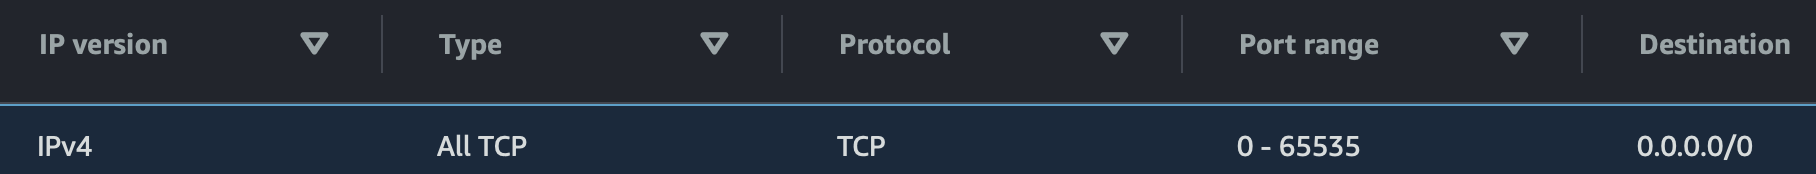
\includegraphics[width=\textwidth]{securityGroup2}
            \caption{security Group 2, TCP in uscita}
            \label{fig:sec2}
        \end{figure}
    \end{itemize}
\end{enumerate}


Una volta creata la macchina avremo la possibilità di scaricare la chiave privata con formato *.pem che useremo per connetterci tramite ssh alla shell della macchina
% [caption=connessione ssh]
% \lstinline{}
\begin{lstlisting}
    ssh -i key.pem admin@*.compute.amazonaws.com
\end{lstlisting}

La primissima operazione sarà l'aggiornamento dei repository e del sistema
% [caption=aggiornamento sistema]
\begin{lstlisting}
    sudo apt update && sudo apt full-upgrade -y
\end{lstlisting}

Poi installiamo il web server nginx che abbiamo analizzato prima
%[caption=Installazione Nginx]
\begin{lstlisting}
    sudo apt install nginx
\end{lstlisting}

Una volta completata l'installazione il web server è già avviato e in ascolto sulla porta 80 \\

Per installare tor è innanzitutto necessario installare \textbf{apt-transport-https} per utilizzare i repository tramite https
\begin{lstlisting}
    sudo apt install apt-transport-https
\end{lstlisting}
Poi aggiungiamo i repository TOR nella cartella \lstinline{/etc/apt/sources.list.d} \\
Dal comando \lstinline{lsb_release -c} possiamo vedere la distribuzione corrente e inserire il repository corretto nella configurazione, con Debian 11 siamo su di una distrubuzione bullseye, creiamo un file chiamato tor.list \footnote{Il nome è configurabile} con le seguenti righe
\begin{lstlisting}
    deb [signed-by=/usr/share/keyrings/tor-archive-keyring.gpg] https://deb.torproject.org/torproject.org bullseye main
    deb-src [signed-by=/usr/share/keyrings/tor-archive-keyring.gpg] https://deb.torproject.org/torproject.org bullseye main
\end{lstlisting}
Assicuriamoci che gpg sia installato nel sistema prima di aggiungere le chiavi
\begin{lstlisting}
    sudo apt install gpg
\end{lstlisting}
Aggiungiamo le chiavi gpg della repository appena creata
\begin{lstlisting}
    wget -qO- https://deb.torproject.org/torproject.org/A3C4F0F979CAA22CDBA8F512EE8CBC9E886DDD89.asc | gpg --dearmor | tee /usr/share/keyrings/tor-archive-keyring.gpg >/dev/null
\end{lstlisting}
Aggiorniamo gli index ed installiamo finalmente tor
\begin{lstlisting}
    sudo apt update && sudo apt install tor -y 
\end{lstlisting} \cite{TorRepo}
Generiamo il torrc file che ci servirà per impostare tutti i parametri di configurazione 
\begin{lstlisting}
    sudo tor -f /etc/tor/torrc
\end{lstlisting}
Apriamo il file e togliamo il commento alle righe \lstinline{HiddenServicePort 80 127.0.0.1:80} e \lstinline{HiddenServiceDir /var/lib/tor/hidden_service}, il primo indica che il traffico arrivato dalla porta virtuale (80) viene reindirizzato alla porta 80 del localhost, ovvero la porta in cui è in ascolto il web server nginx, il secondo ci serve per indicare la directory in cui si trova l'hostname del sito e le chiavi crittografiche. \\
Riavviamo tor per aggiornare la configurazione, assicurarci che il file torrc non contenga errori e che il sistema sia funzionante
% HiddenServiceDir /var/lib/tor/hidden_service/
\begin{lstlisting}
    sudo systemctl restart tor
\end{lstlisting}

\subsection{Gestire la comunicazione tramite i socket unix}

A questo punto tor ha creato gli introduction points e ha generato un circuito con ognuno di essi, ha generato le chiavi ed il proprio hostname, queste informazioni sono state aggiunte nella cartella che abbiamo inserito nell'HiddenServicePort, in particolare hostname contiene l'indirizzo tor del nostro servizio \cite{SetupOnionService} \\
Questo sistema però non è completamente sicuro, stiamo collegando tor con il web server tramite una porta, essendo entrambi i processi sulla stessa macchina il sistema ottimale è utilizzare un socket unix tra i due processi. Questo impedisce ad un utente non Tor di accedere direttamente al web server senza dover configurare firewall che comunque aggiungono complessità nella rete \\
Apriamo il file \lstinline{/etc/nginx/sites-enabled/default} e nella sezione server aggiungiamo il socket in ascolto, cosi che la comunicazione possa passare anche per il socket unix
\begin{lstlisting}
    listen unix:/var/run/website.sock;
\end{lstlisting}
Possiamo inoltre rimuovere la connessione dalla porta 80 commentando le seguenti righe
\begin{lstlisting}
    #listen 80 default_server;
    #listen [::]:80 default_server;
\end{lstlisting}
Dopo aver riavviato nginx ed esserci assicurati che non vi siano errori apriamo il file torrc e inseriamo lo stesso socket
\begin{lstlisting}
    HiddenServicePort 80 unix:/var/run/website.sock
\end{lstlisting}
Infine riavviamo tor, se tutto è andato a buon fine il servizio dovrebbe essere in grado di rispondere
\begin{lstlisting}
    sudo systemctl restart tor
\end{lstlisting}

\importImage{
    \label{fig:nginxConnection} 
    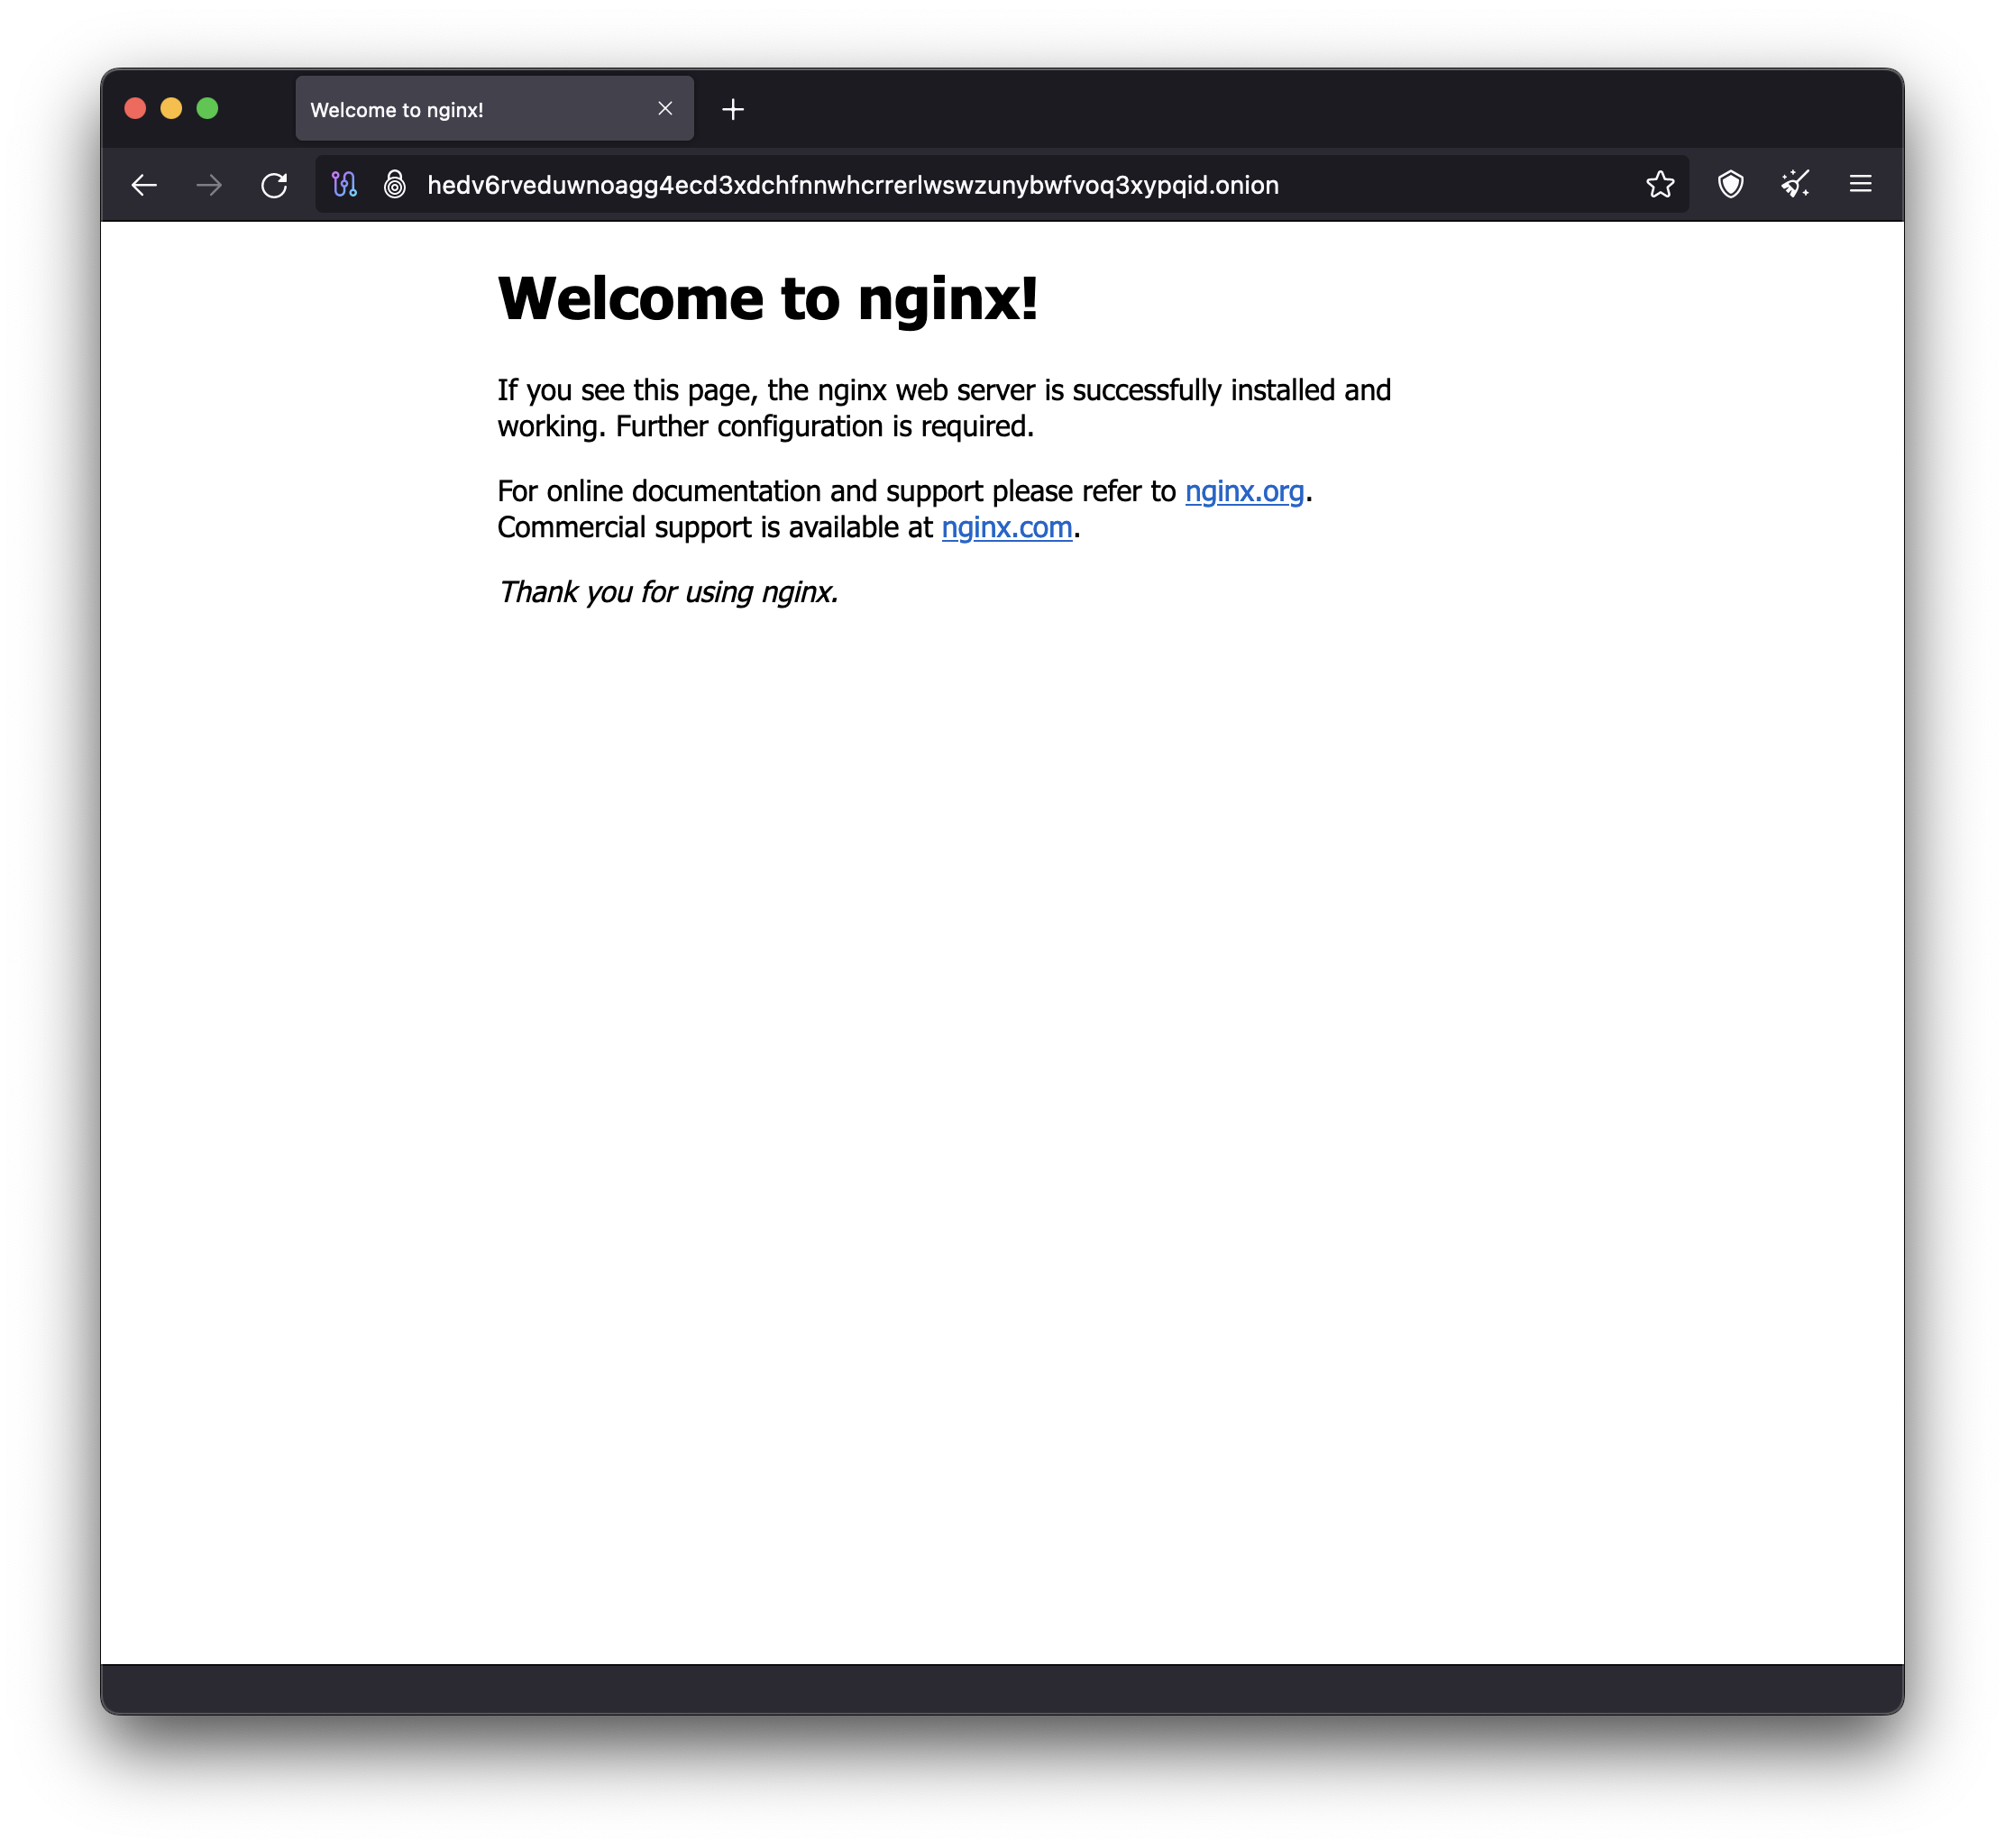
\includegraphics[width=\textwidth]{connectionSucceeded}
    \caption{Connessione al web server nginx}
}

\newpage
\subsection{Creazione di un url personalizzato}
Ora che il servizio è attivo e disponibile possiamo iniziare a configurarlo a nostro piacimento, la prima cosa che potremmo voler fare è cambiare l'hostname impostandone uno personalizzato, almeno in parte, un'esempio è il sito email di proton \textbf{protonmail}rmez3lotccipshtkleegetolb73fuirgj7r4o4vfu7ozyd.onion \\
Vi sono diversi strumenti per fare quest'operazione, si sfrutta la tecnica del brute force per generare chiavi ed indirizzi casuali fino a trovarne uno inizia con il termine che abbiamo scelto, potrebbe impiegare diverso tempo ed è consigliabile usare un computer più potente della nostra macchina virtuale. 
Per questa implementazione useremo il tool mkp224o \cite{V3AddressGeneratorRepo}, possiamo installarlo su linux o usarlo su windows da riga di comando semplicemente indicando il nome con cui dovrà iniziare

\footnote{Il file viene avviato direttamente dalla cartella del sorgente, per cui apponiamo \lstinline{./}}
\begin{lstlisting}
    ./mkp224o tesilm
\end{lstlisting}
    
Da notare che più caratteri si scelgono nel matching più il software impiegerà nella generazione di un dominio. Otteniamo il nuovo indirizzo del server\footnote{tesilm3jb64lw3upj4uu5fsxi2nrtbhbhkbu2dsbn46qka7j4kf7peqd.onion} con le relative chiavi \\
Possiamo copiarle sul server con scp usando l'opzione -i per definire il file d'identità, come facciamo con ssh
    
\begin{lstlisting}
    cd tesilm3jb64lw3upj4uu5fsxi2nrtbhbhkbu2dsbn46qka7j4kf7peqd.onion
    scp -i key.pem * admin@*.compute.amazonaws.com:~/var/lib/tor/hidden_service
\end{lstlisting}

Avviamo la connessione al server e riavviamo tor per impostare le modifiche

\importImage{
    \label{fig:mkpCommandOut} 
    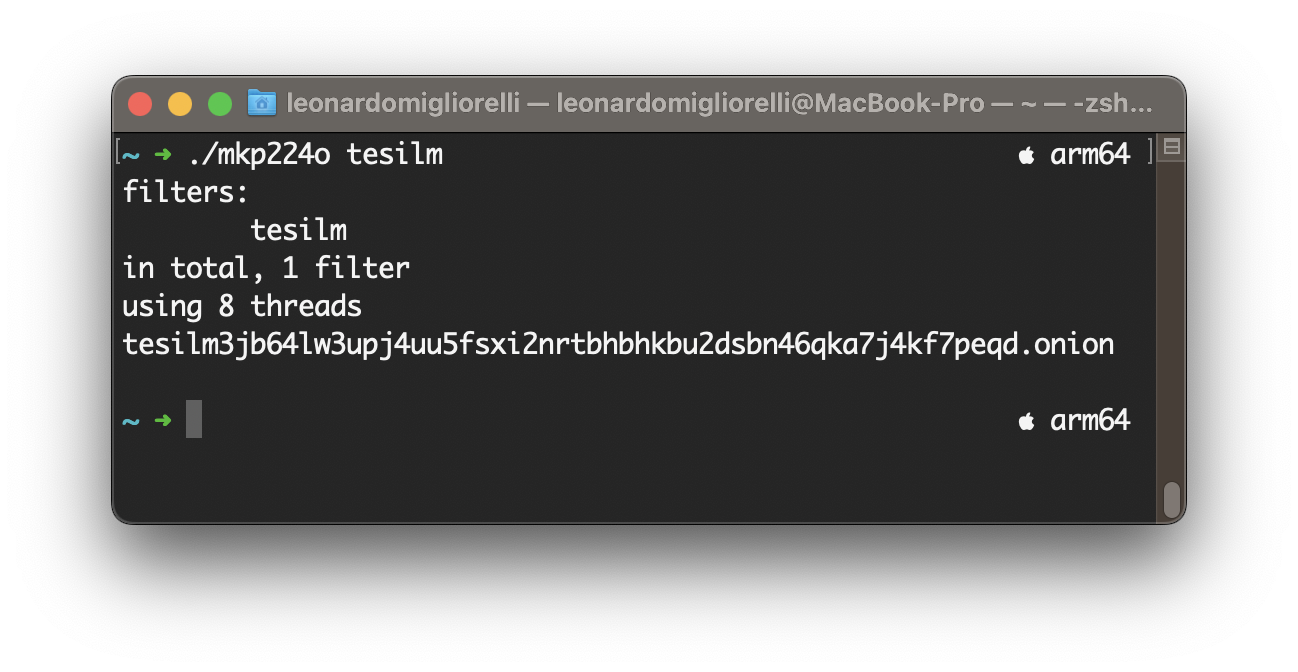
\includegraphics[width=\textwidth]{mkpCommandOut}
    \caption{Comando mkp224o e output}
}

\importImage{
    \label{fig:customAddressConnection} 
    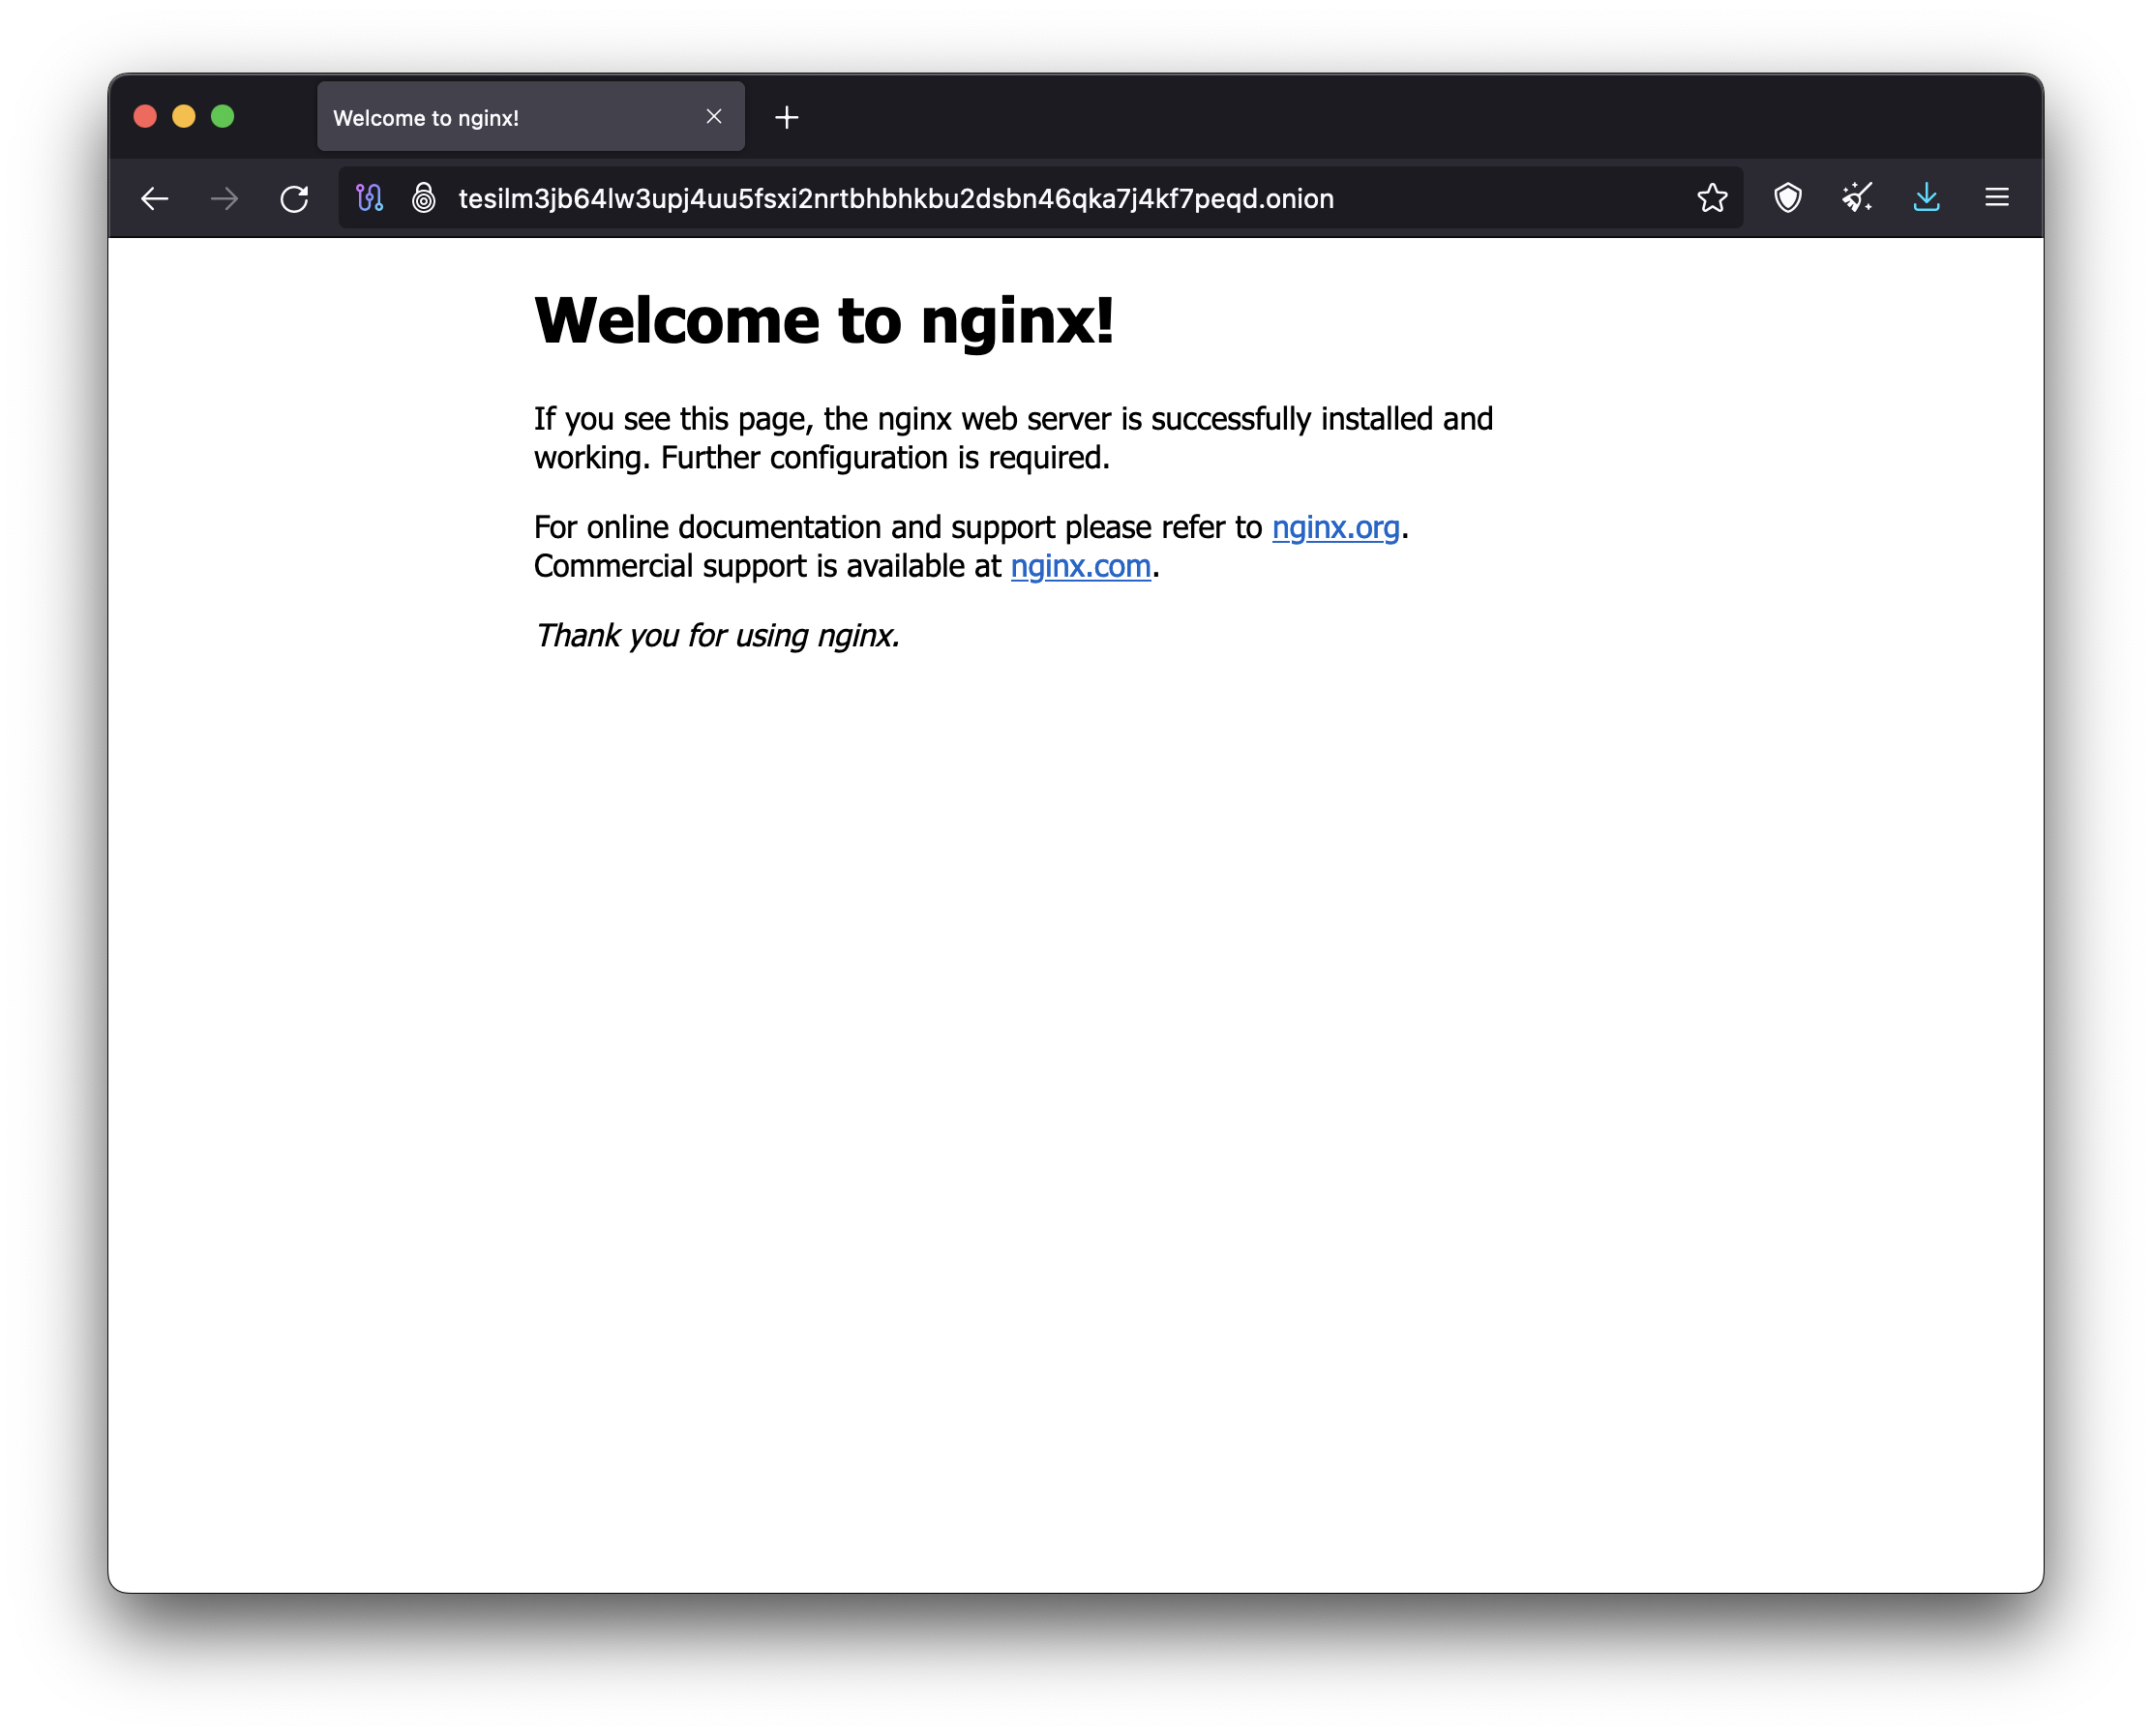
\includegraphics[width=\textwidth]{connectionCustomAddress}
    \caption{Connessione con il nuovo url}
}

\newpage

\subsection{Far conoscere il sito}
Un'altra caratteristica importante per ogni sito è la capacità di essere ricercato tramite un motore di ricerca, ci sono diversi motori che eseguono l'indexing. Tra questi c'è notevil\footnote{http://notevilmtxf25uw7tskqxj6njlpebyrmlrerfv5hc4tuq7c7hilbyiqd.onion} funziona come un classico motore di ricerca, a differenza di altri motori come Torch che invece esegue la ricerca più in base al contenuto che all'url\footnote{Un test di ricerca di 'proton mail' in entrambi mostra solo notEvil restituirci il sito corretto} \\
In NotEvil è possibile contattare gli amministratori del motore per richiedere l'aggiunta di un sito. Dalla pagina ufficiale è infatti presente il pulsante di contatto, dopo un breve controllo ci permette di inviare una richiesta anonima cosi che il sito possa essere analizzato ed aggiunto\\
Un'altro sistema per far conoscere il sito agli utenti finali è l'utilizzo di siti specializzati come OnionDir\footnote{https://oniondiricuc4x2y5qbucg4jyp2ael5rxy7aahy5f4fbars2jkkf7vad.onion.nz} che permette di aggiungere il proprio sito in maniera completamente anonima. \\
In questo caso basta cliccare sul tasto \lstinline{Add Link} nella toolbar in alto. \\
\importImage{
    \label{fig:OnionDir}
    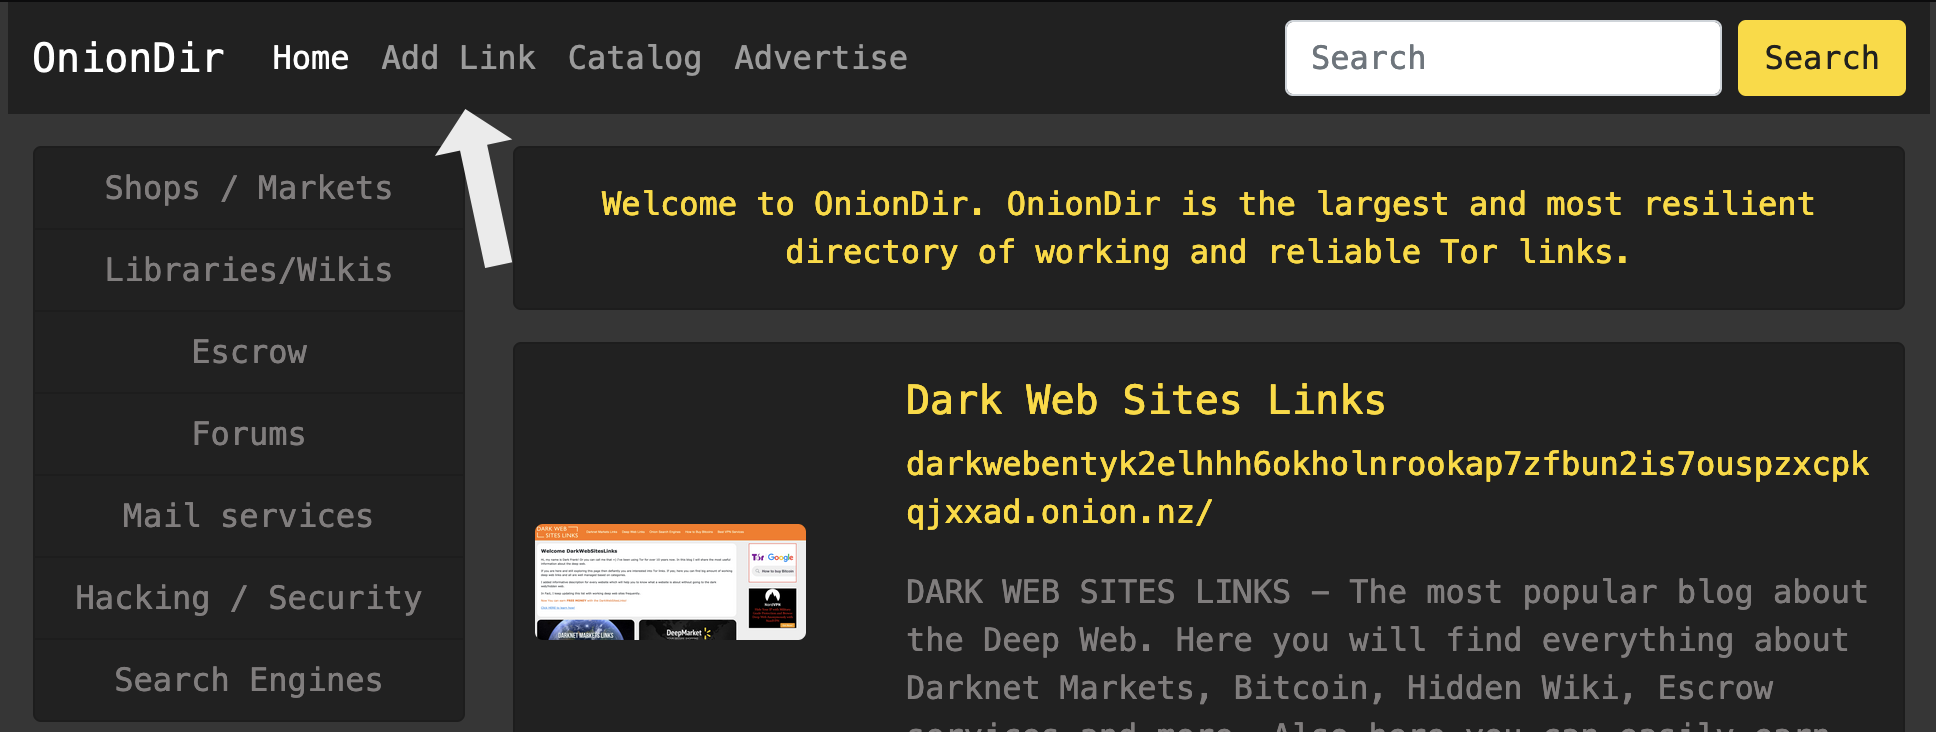
\includegraphics[width=\textwidth]{OnionDirMain}
    \caption{OnionDir, Pagina iniziale}
}
A questo punto possiamo inserire l'url e una piccola descrizione, come NotEvil il sito sarà scansionato per evitare truffe o contenuti proibiti, come indicato nelle poche righe di descrizione dei termini del servizio. \\
\importImage{
    \label{fig:OnionDirForm}
    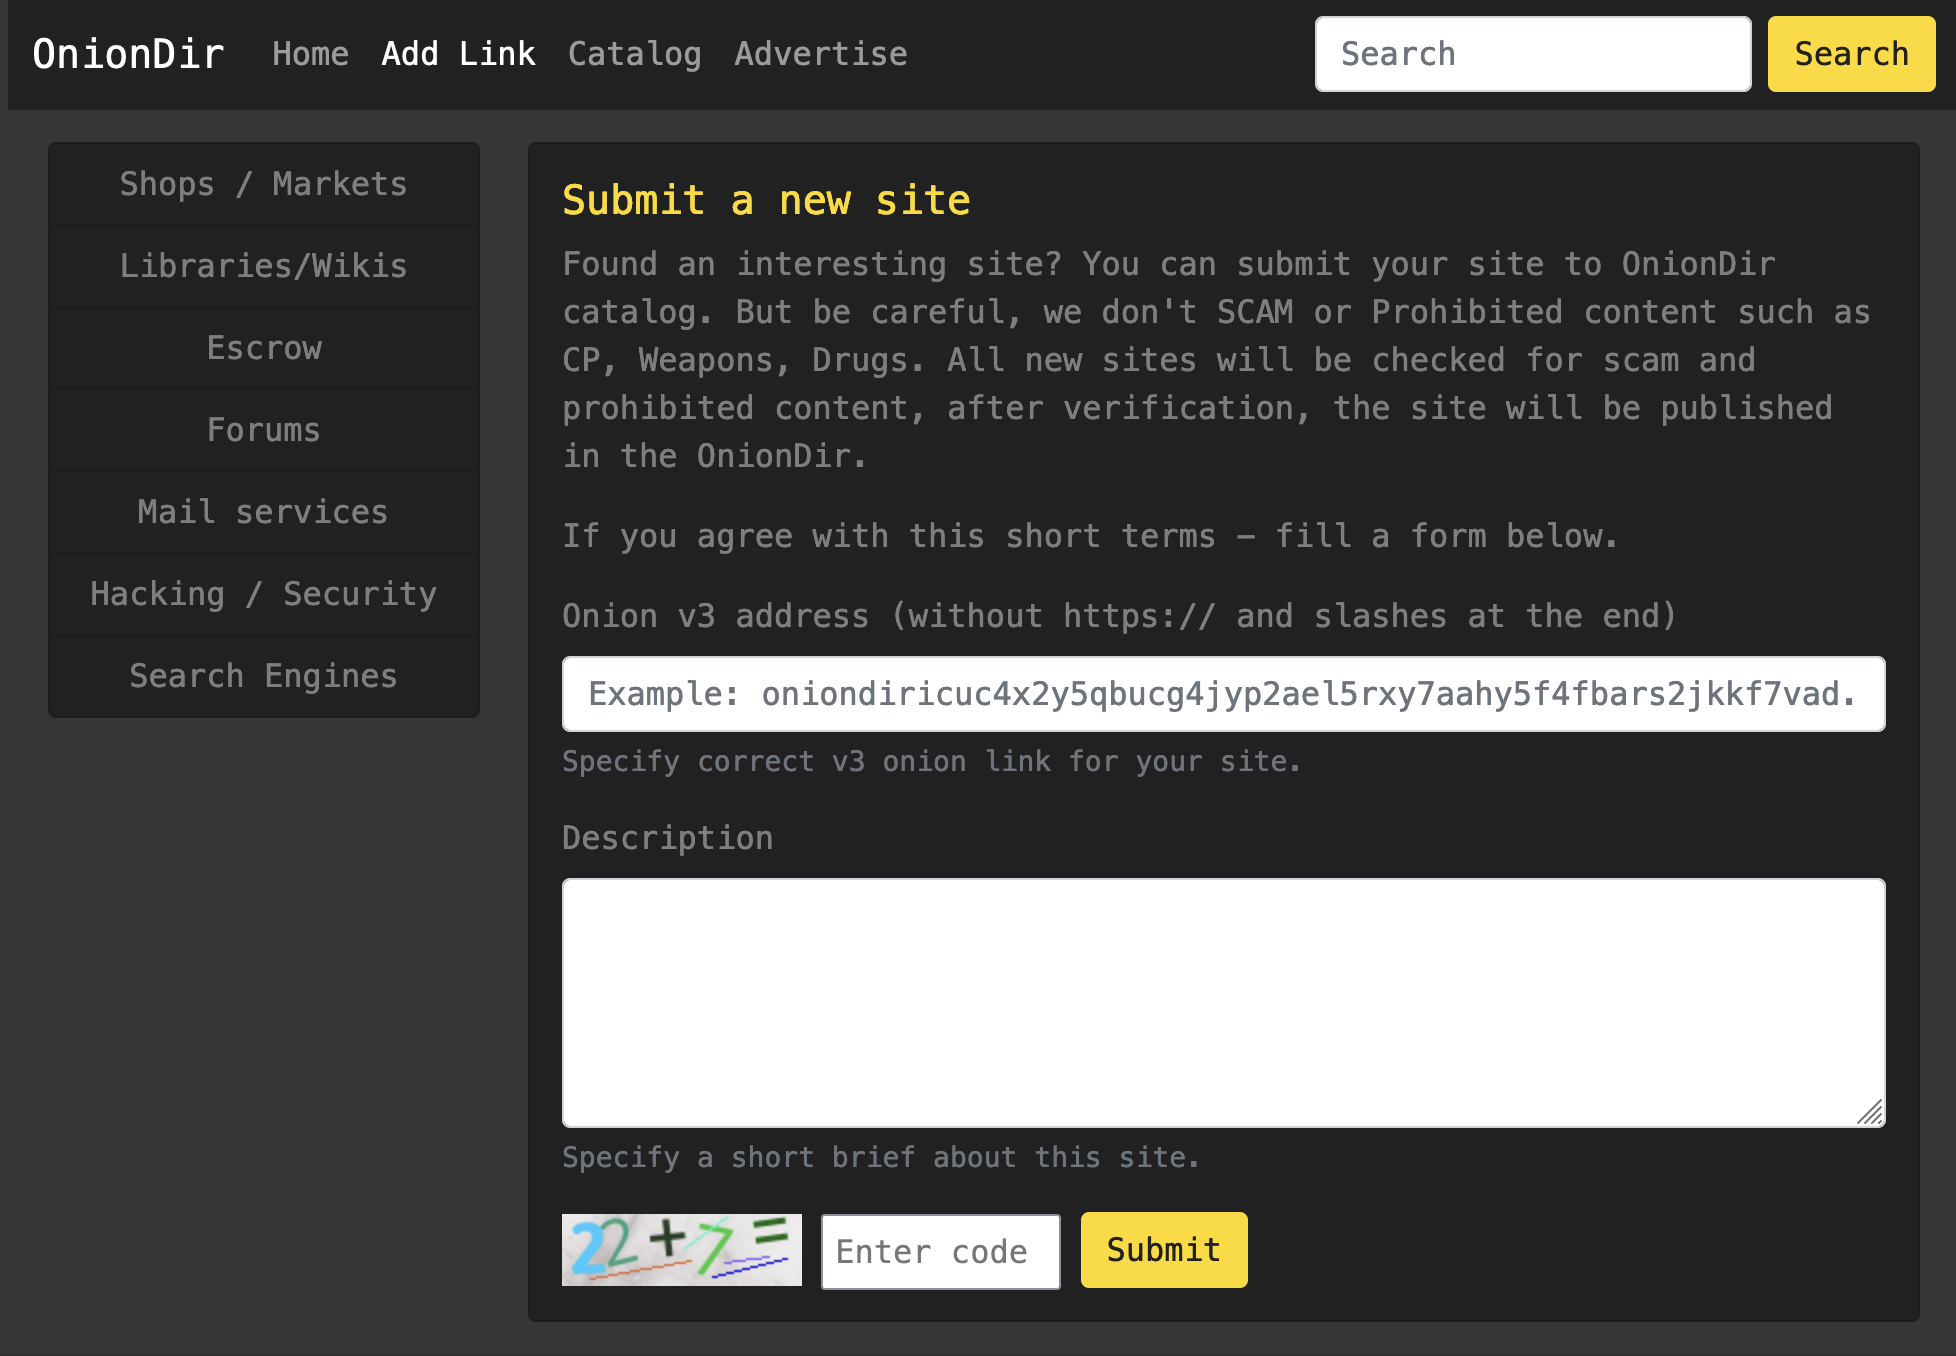
\includegraphics[width=\textwidth]{OnionDirForm}
    \caption{OnionDir, Form aggiunta sito}
}